%%% TITLE %%%
\title{\Large \bf Canalization of the evolutionary trajectory of the human influenza virus}
\maketitle

\begin{abstract}
\noindent Influenza A (H3N2) has persisted in the human population since 1968 through continued seasonal epidemics.  During this time, the influenza virus underwent substantial antigenic drift, allowing it to infect a large fraction of the human population year after year.  Understanding the process of antigenic evolution is key to our efforts of disease control and surveillance; the continual emergence of new antigenic variants requires corresponding updates to the influenza vaccine.  The antigenic evolution of H3N2 influenza has been experimentally characterized, resulting in an two-dimensional `antigenic map' describing antigenic similarity and distance between strains.  The genetic relationships among H3N2 strains have also been distinguished, showing a characteristic ladder-like genealogical tree.  This work seeks to simultaneously model epidemiological, antigenic, genealogical and spatial patterns of the influenza virus.  Here, we use a large-scale individual-based model to show that evolution in a Euclidean antigenic space results a close correspondence between model behavior and available data in terms of antigenic map and in terms of genealogical tree.  We find a human immunity results in rapid population turnover in the influenza virus and that this population turnover occurs primarily along a single antigenic axis.  Thus, selective dynamics induce a canalized evolutionary trajectory, preceding as rapidly as possible away from human immune history.  Owing to these selective dynamics, we find the evolutionary fate of influenza population to be surprisingly repeatable and hence, in theory, predictable.
\end{abstract}

Epidemic influenza is responsible for between 250,000 and 500,000 global deaths annually, with influenza A (H3N2) having historically caused the bulk of human mortality and morbidity \cite{flufactsheet}.  Influenza A (H3N2) has continually circulated within the human population since its introduction in 1968, exhibiting recurrent seasonal epidemics in temperate regions and less periodic transmission in the tropics.  Annual winter epidemics of H3N2 influenza show average cumulative attack rates of 3--8\% \cite{Monto93,Koelle09}.  Since its emergence, influenza A H3N2 has continually evolved both genetically and antigenically.  Most antigenic drift is thought to be driven by changes to epitopes in the hemagglutinin (HA) protein \cite{Nelson07NatRevGenet}.  Phylogenetic analysis of the genetic relationships among HA sequences has revealed a distinctive genealogical tree showing a single predominant trunk lineage and side branches that persist for only 1--5 years before going extinct \cite{Fitch97}.  This tree shape is indicative of serial replacement of strains over time; H3N2 influenza shows rapid evolution, but low standing genetic diversity.

This observation has remained puzzling from an epidemiological standpoint.  Antigenic evolution occurs rapidly and strong diversifying selection exists to escape from human immunity; why then do we see serial replacement of strains rather than continual accumulation of antigenic and genetic diversity?  Indeed, simple epidemiological models show explosive diversity of genotype and phenotype over time \cite{Ferguson03,Tria05}.  Previous work has sought model-based explanations of the limited diversity of influenza, relying on short-lived strain-transcending immunity \cite{Ferguson03,Tria05}, complex genotype-to-phenotype maps \cite{Koelle06} or a limited repertoire of antigenic phenotypes \cite{Recker07}. 

Fortunately, experimental characterization of antigenic phenotype is possible through the hemagglutination inhibition (HI) assay, which measures the cross-reactivity of HA from one virus strain to serum raised against the another strain \cite{Hirst43}.  The results of many HI assays across a multitude of virus strains can be combined to yield a two-dimensional map, representing antigenic similarity and distance as an easily visualized and quantified measure \cite{Smith04}.  The path traced across this map by influenza A (H3N2) from 1968 until present is largely linear, showing serial replacement of one strain by another; there are no major bifurcations of antigenic phenotype \cite{Smith04}.  The genetic and antigenic patterns of H3N2 influenza appear consistent; both antigenic map and genealogical tree lack branching events wherein separate lineages of influenza move in different antigenic/genetic directions.

Herein, we seek to further reconcile antigenic and genetic patterns of influenza evolution using a large-scale individual-based model.  Our approach seeks to simultaneously and directly model the antigenic map and genealogical tree of the global influenza population.  Additionally, our model incorporates geographic population structure, elucidating broad patterns of migration between regions with contrasting seasonal dynamics.

Using a dimensionality reduction approach, Smith and colleagues \cite{Smith04} show that a two-dimensional map adequately explains observed antigenic distances between strains.  Our model begins with this basic finding.  Here, in an analogous fashion, antigenic phenotypes are represented geometrically as points on a plane.  After exposure to a virus, a host's risk of infection is proportional to the Euclidean distance between the infecting phenotype and the closest phenotype in the host's immune history.  Virus strains possessing antigenically novel phenotypes will have a transmission advantage compared to strains whose phenotypes are more similar to phenotypes present in host immune histories.  Mutations pertub antigenic phenotype, moving phenotype in a random radial direction and for a randomly distributed distance.  This distribution is parameterized so that mutation usually has little effect on antigenic phenotype, but occasionally has a large effect.  This is similar to the neutral networks implemented by Koelle et al. \cite{Koelle06}, wherein most amino acid changes result in little decrease to cross-immunity between strains, but some changes result in large jumps in cross-immunity.

We implemented this geometrical model in a large-scale individual-based simulation intended to describe global patterns of influenza epidemiology and evolution (for details see \textsl{Methods}).  The simulation includes multiple host populations with different seasonal forcings, hosts with complete immune histories of infection, and viruses with antigenic phenotypes.  As the simulation proceeds, infections are tracked and a complete genealogy connecting virus samples is constructed.  This avoids the messy intermediate step of phylogenetic inference common to phylodynamic simulations.  Results shown here are for a single simulation of 40 years of virus evolution in a population of 90 million hosts.  

The virus persists over the course of the 40-year simulation, infecting a significant fraction of the host population through annual winter epidemics in temperate regions and through less periodic epidemics in the tropics (Fig.~\ref{incmaptree}A).  Across replicate simulations, we observe average yearly attack rates of 6.8\% in the temperate regions and rates of 7.1\% in the tropics.  Over the course of the simulation, the virus population evolves in antigenic phenotype (Fig.~\ref{incmaptree}B, Fig.~\ref{phenotypes}A).  Mutations move virus phenotypes in antigenic space and the resulting novel phenotypes outcompete older `spent' virus phenotypes.  There are a handful of highly abundant phenotypes sampled repeatedly and a large number of phenotypes appearing a low abundance (Fig.~\ref{phenotypes}A).  These low abundance phenotypes form clouds around the high abundance phenotypes from which they arise.  The appearance of the clusters in the antigenic map (Fig.~\ref{incmaptree}B) come from the regular spacing of high abundance phenotypes (Fig.~\ref{phenotypes}A) combined with experimental measurement noise (see \textsl{Methods}).  Over the course of the simulation, clusters of antigenically similar strains are replaced by novel clusters of more advanced strains (Fig.~\ref{incmaptree}B, Fig.~\ref{phenotypes}B).  

Remarkably, although antigenic phenotype is free to mutate in any direction in the two-dimensional space, selection pressures force the virus population to move in nearly a straight line in antigenic space (Fig.~\ref{incmaptree}B, Fig.~\ref{phenotypes}A).  Across replicate simulations, 94\% (interquartile range 92--98\%) of the variance of antigenic phenotype can be explained by a single dimension of variation.  This mirrors the empirical results showing a largely linear antigenic map for H3N2 influenza isolates from 1968 to 2003 \cite{Smith04}.  Because of the primarily one-dimensional movement, antigenic distance from the original phenotype increases linearly with time (Fig.~\ref{phenotypes}C).  Antigenic evolution occurs in a punctuated fashion; periods of relative stasis are interspersed with more rapid antigenic change leading to a fundamental linkage of evolutionary and epidemiological dynamics (see \textsl{Supporting Text}).

\subsection*{Evolutionary dynamics}

The genealogical tree connecting the evolving virus population appears characteristically sparse with pronounced trunk and short-lived side branches  (Fig.~\ref{incmaptree}C).  This tree shape is reflected in low levels of standing diversity; an average of 5.68 years of evolution separate two randomly sampled viruses in the population.  This level of diversity matches what is observed in phylogenies of influenza A (H3N2) \cite{Rambaut08}.  We find that diversity commonly increases during periods of relative evolutionary stasis (when the population remains within an antigenic cluster) and contracts during periods of antigenic drift (during cluster transition events) (Fig.~\ref{incmaptree}C).  A spindly genealogical tree is indicative of population turnover.  Novel antigenic phenotypes continually replace more primitive `spent' phenotypes, purging their genealogical diversity.  Strong selective pressure results in rapid antigenic drift and reduced effective population size \cite{BedfordTreeTopology}.

Selective pressures can be examined by comparing which mutations fix, i.e.\ are incorporated into the progenitor trunk lineage, and which mutations are lost, i.e.\ incorporated into side branches bound for extinction.  This approach has shown that, in influenza A (H3N2), natural selection promotes mutations to epitope sites in the HA1 region \cite{Bush99MBE,Wolf06,Bhatt11}.  In the present case, we compare mutational patterns on trunk branches to mutational patterns on side branches (Table~\ref{mktable}).  We find evidence for pervasive positive selection for antigenic change.  Trunk lineages show increased rates of phenotypic mutations (13.23$\times$), increased effect size of mutations that do occur (1.99$\times$) and, in combination, much increased rates of antigenic drift (26.25$\times$).  Trunk mutations tend to push antigenic phenotype forward along the line of primary antigenic variation (Fig.~\ref{mutspectrum}).  

Thus, lineages harboring mutations that push antigenic phenotype forward are likely to become progenitor lineages, and may be identified prospectively.  This insight forms a large part of the basis of the World Health Organization vaccine strain selection program \cite{Barr10}.  We find a roughly linear relationship between the antigenic effect of a mutation and likelihood of this mutation becoming incorporated into the trunk (Fig.~\ref{probtrunk}).

\subsection*{Spatial dynamics}

The genealogical tree also contains detailed information on the history of migration between regions.  We find that, consistent with empirical estimates \cite{Russell08,Bedford10}, the trunk resides primarily within the tropics, where seasonal dynamics are less prevalent (Fig.~\ref{spatial}A).  Across replicate simulations, we observe that 72\% of the trunk's history is in the tropics, 14\% is in the north and 14\% is in the south.  Because host contact rates between regions are symmetrical and host population sizes are equivalent, without seasonal forcing, we would expect trunk proportions of one third for each region.  The observed asymmetry can be explained by strong seasonal dynamics (Fig.~\ref{incmaptree}A), wherein temperate epidemics are bound for regional extinction at the end of the winter season.  In order for a lineage to be part of the trunk and pass through a temperate region, a migration event into the temperate region at the beginning of the season and a subsequent migration event out of the temperate region before the end of the season is required. 

However, it's apparent from the genealogy that migration events between temperate regions and from temperate regions into the tropics are relatively common (Fig.~\ref{spatial}A).  Thus, it appears that all combinations of migration events occur, but migration events out of the tropics result in evolutionary dead ends.  We calculated rates of migration based on observed event counts and branch length opportunity across replicate simulations, separating region-specific rates on side branches (Fig.~\ref{spatial}B) from region-specific rates on trunk branches (Fig.~\ref{spatial}C).  We find that migration patterns on side branches are close to symmetric, with fairly equal rates between all regions (Fig.~\ref{spatial}B).  Extrapolating from these migration rates, we would expect a stationary distribution of 38\% north, 38\% south and 24\% tropics.  It appears that upon leaving the trunk, lineages have a slight preference to move to temperate regions.  However, migration patterns on trunk branches are highly asymmetric, with high rates of movement between temperate regions and from temperate regions into the tropics; trunk lineages rarely leave the tropics once they arrive there (Fig.~\ref{spatial}C).  Extrapolating from these rates, we arrive at an expected stationary distribution of 76\% tropics and 24\% temperate regions, in line with the observed proportion of trunk residing in the tropics.

It may at first seem counter-intuitive to see higher rates of movement from the temperate regions into the tropics along trunk branches, but it makes sense when thought of in terms of conditional probability.  Only those lineages that migrate into the tropics or those lineages which rapidly migrate between the north and south have a chance at becoming the trunk lineage, while lineages that remain within the temperate regions are doomed to extinction.  These results suggest a possible resolution to an apparent discrepancy in analyses of the global migration patterns of influenza.  Russell et al.\ \cite{Russell08} emphasize a source-sink model of movement the HA protein of influenza A (H3N2) based on their finding of a trunk lineage residing within China and the Southeast Asian tropics.  Whereas, Bedford et al.\ \cite{Bedford10} emphasize a global metapopulation model based on phylogenetic inference of migration rates across the entire tree.  We find that both scenarios are simultaneously possible; side branches may be highly volatile moving rapidly and symmetrically between regions, while the trunk lineage may be more stable remaining within a region (or within a highly connected network of regions) that has more persistent transmission.  In light of these results, we suggest that future work on the phylogeography of influenza take into account trunk vs.\ side branch differences in migration patterns.

\subsection*{Reconciling model and data}

We find a remarkable correspondence between the antigenic and genealogical patterns generated by our model (Fig.~\ref{incmaptree}B--C) and patterns of genetic and antigenic evolution exhibited by influenza A (H3N2) \cite{Fitch97,Smith04}.  

Multiple epidemiological/evolutionary mechanisms have been proposed to explain the restricted genetic diversity and rapid population turnover of influenza A (H3N2) \cite{Ferguson03,Tria05,Koelle06,Recker07}.  It remains a central question as to the extent that short-lived strain-transcending immunity is responsible for influenza's limited diversity and spindly genealogical tree.  Our findings suggest a possible resolution.  Although lacking short-lived immunity, our model shows a detailed correspondence to both the antigenic map and genealogical tree of H3N2 influenza.  If an antigenic map were to show a deep bifurcation, where two viral lineages move in different antigenic directions, then we would expect the same bifurcation to be evident in the genealogical tree.  Short-lived strain-transcending immunity provides a mechanism by which lineages may diverge in antigenic phenotype, but still interfere with one another.  This mechanism would explain a situation where bifurcations emerge in the antigenic map, but competition results in the extinctions of divergent antigenic lineages.  The empirical antigenic map \cite{Smith04} suggests that this is not the case; one cluster leads to another cluster in orderly succession and there is never competition between two antigenically novel clusters.  This supports the hypothesis that antigenic evolution is primarily limited by a lack of mutational input.  This is not to say that short-lived strain-transcending immunity is not present; observed interference between subtypes \cite{Ferguson03,Goldstein11} provides substantial evidence for its existence.  Instead, we suggest that short-lived strain-transcending immunity does not automatically generate antigenic maps and genealogical trees consistent with empirical evidence.

\subsection*{Canalization of evolutionary trajectory}

The virus population consistently moves in a linear trajectory through antigenic space.  It would seem possible for one viral lineage to move in one antigenic direction, while another lineage moves tangentially, eventually resulting in two non-interacting viral lineages.  Instead, only movement in a single antigenic direction is favored.  The origins of this pattern can be seen in the interaction between virus evolution and host immunity (Fig.~\ref{immunity}).  As the virus population evolves forward it leaves a wake of immunity in the host population.  At the end of the simulation several virus phenotypes exist with similar antigenic locations; all of these phenotypes lie significantly ahead of the peak of host immunity (Fig.~\ref{immunity}).  It can be seen that mutations of a specific magnitude will be more successful (in terms of having a higher risk of infection) if they continue forward along the path the virus has been taking.  From competition for susceptible hosts, those viruses that are furthest ahead on this line will have a transmission advantage over viruses that lag behind or harbor tangential mutations.  The differential success of these leading viruses results in antigenic drift of the virus population (Fig.~\ref{phenotypes}) and its rapid turnover (Fig.~\ref{incmaptree}C).  Thus, we see that natural selection results in the canalization of the antigenic evolution of the viral population; where mutation provides multiple avenues of evolutionary change, selection `chooses' but one.

After the work of Smith and colleagues \cite{Smith04}, it remained an open question of why a two-dimensional map should explain the antigenic trajectory of H3N2 influenza.  Although the authors astutely speculated that ``there is a selective advantage for clusters that move away linearly from previous clusters as they most effectively escape existing population-level immunity, and this is a plausible explanation for the somewhat linear antigenic evolution in regions of the antigenic map.''  This hypothesis remained to be tested.  Here, we show from a simple model of epidemiology and evolution that a linear trajectory of antigenic evolution dynamically emerges due the selective pressures on the virus population.  This result simultaneously explains the linear pattern of antigenic drift \cite{Smith04} and the characteristically spindly genealogical tree \cite{Fitch97} exhibited by influenza A (H3N2).

Still, we were uncertain to what extent these results were contingent on the dimensionality of the underlying antigenic model.  Selecting a `line' of movement from `circles' of mutation seems an easier proposition that selecting a `line' of movement from hyperspheres of mutation.  If mutation can push antigenic phenotype in a large number of dimensions, does selection still constrain the movement of the virus population to a mostly one-dimensional manifold within this higher dimensional space?  We tested this by implemented our model in a 10-dimensional antigenic space.  Here, mutations occur as 10-spheres, but the distribution of Euclidean distances moved by a mutation is exactly the same as in the previous two-dimensional model formulation.  We arrive at nearly the same results with this model; principal components analysis shows that the first dimension of variation accounts for 87\% of the total variance (Fig.~\ref{10dgrid}).  The second dimension accounts for 7\% of the variance, the third dimension accounts for 2\% and each additional dimension accounts for less than 1\% of the overall variance.  Thus, even if the underlying mutational space of H3N2 influenza were high dimensional, we would still expect to find a two-dimensional antigenic map sufficient to explain observed antigenic relationships among strains.  These results support the linear structure of the antigenic map of Smith et al.\ \cite{Smith04} as firm reality as opposed to an artifact arising from censored sampling procedures \cite{Recker07}.

Additionally, we examined the timing of phenotypic mutations along the trunk of the genealogy.  We found that mutations occurred at surprisingly regular intervals, with significantly less variation of waiting times than expected under a simple random process (Fig.~\ref{waittimes}).  Under a Poisson process of constant rate, the coefficient of variation (defined as $\sigma / \mu$) is expected to equal 1 (unity).  However, across replicate simulations we observe a mean coefficient of variation of 0.66  (interquartile range 0.54--0.75), significantly less than the random expectation ($P = 6.7 \times 10^{-15}$, Wilcoxon signed-rank test).  There is a relative scarcity of mutation events occurring in intervals under 1 year and a relative excess of a mutation events occurring in 2--3 year intervals (Fig.~\ref{waittimes}).  Observed cluster transition events show a similar pattern, occurring most commonly in 2--3 year intervals and showing a coefficient of variation of 0.56.  Thus, we find considerable regularity in terms of the direction of antigenic movement, but also in the timing of antigenic transitions.  

\subsection*{Repeatability of evolution}

It seems clear that selection for antigenic novelty reduces the degrees of freedom of antigenic evolution.  In light of this, we wanted to examine the degree of stochasticity in replicated evolutionary trajectories, and thereby test what happens when we ``wind back the tape'' \cite{GouldWonderfulLife} on the evolution of the virus.  We ran 100 replicate simulations, each starting from the endpoint of the original 40-year simulation (Fig.~\ref{replicateevol}).  Initially, we find a great detail of repeatability.  During the first year of evolution, every replicate virus population undergoes an antigenic transition, moving an average of 3.0 units away from the initial population mean.  Additionally, every replicate population moves in roughly the same direction, so that the resulting antigenic locations differ little across replicates (Fig.~\ref{replicateevol}).  After two years of evolution, there is still little variation in evolutionary trajectory across replicates.  Though from years 3 to 5 there is growing dissimilarity between replicates, so that at the end of 5 years, replicate populations differ substantially (Fig.~\ref{replicateevol}).  This 1--2 year timescale of repeatability can be explained by the presence of standing antigenic variation.  In the initial virus population, there are 5 novel antigenic variants present with a combined frequency of 10.5\% (Fig.~\ref{replicateevol}).  Without fail, one of these novel antigenic variants comes to take over the virus population.  This consistent antigenic transition results in a repeatable peak in northern hemisphere incidence across replicates (Fig.~\ref{replicatetimeseries}).  The following year (year 2) appears refractory, showing low northern hemisphere incidence across replicates.  After three years, repeatability has mostly disappeared, and incidence is highly variable across replicates (Fig.~\ref{replicatetimeseries}), with further evolution relying on intrinsically stochastic mutational events.

We see that the initial 1--2 year evolutionary trajectory, during which time standing variation plays out, is highly repeatable, and thus predictable given enough information and the right methods of analysis.  However, prediction of longer-term evolutionary scenarios will necessarily be difficult or impossible except in a vague sense.  After 5 years of evolution, replicate simulations show abundant variation in evolutionary trajectory, but in each case there has been movement away from past phenotype, consistent with evolutionary canalization.  Through careful surveillance efforts and genetic and antigenic characterization of influenza strains, the World Health Organization makes twice-yearly vaccine strain recommendations \cite{Barr10}.  It may be possible to combine these sorts of modeling approaches with surveillance data to gauge the likelihood that an apparently novel sampled variant will spread through the population.

\section*{Conclusion}

Recent work on empirical fitness landscapes has shown that natural selection follows few mutational paths \cite{Weinreich06}.  The spindly genealogical tree and serial replacement of influenza strains has remained a puzzling phenomenon.  We suggest that the evolutionary and epidemiological dynamics displayed by the influenza virus may be explained as an outgrowth of selection to avoid host immunity.  Natural selection can only `see' one step ahead, and so sacrifices long-term gains for short-term success.  The result is a canalized evolutionary trajectory lacking antigenic diversifaction.

%%% REFERENCES %%%
\bibliographystyle{plos2009}
\bibliography{/Users/bedfordt/Documents/bedford}

\pagebreak

%%% FIGURES %%%
\section*{Figures}

%%% Figure 1: incmaptree %%%
\begin{figure}[H]
	\centering
	\includegraphics{figures/incmaptree}
	\caption{\textbf{Simulation results showing epidemiological, antigenic and genealogical dynamics}. (A) Weekly timeseries of incidence of viral infection in north and tropics regions. (B) Antigenic map depicting phenotypes of 5943 viruses sampled over the course of the simulation.  To construct the map, noise was added to each sample and the resulting observations grouped into 10 clusters and colored accordingly.  Grid lines show single units of antigenic distance. (C) Genealogical tree depicting the infection history of 376 samples from the virus population.  Parent/offspring relationships were tracked over the course of the simulation, giving a direct observation of the genealogy rather than a phylogenetic inference. Cluster assignments were used to color panels (A), (B) and (C) in a consistent fashion.}
	\label{incmaptree}
\end{figure}

\pagebreak

%%% Figure 2: phenotypes %%%
\begin{figure}[H]
	\centering
	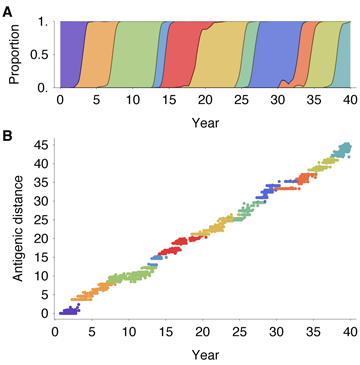
\includegraphics{figures/phenotypes}
	\caption{\textbf{Antigenic evolution over the course of the 40-year simulation}. (A) Two-dimensional antigenic phenotypes of 5943 viruses.  Each discrete virus phenotype is shown as a bubble, with bubble area proportional to the number of times this phenotype was sampled. (B) Proportion of virus population comprised of each antigenic cluster through time.  (C) Antigenic distance from initial phenotype ($x=0,y=0$) for each of 5943 virus samples relative to time of virus sampling. In (A) and (C) viruses were sampled at a constant rate proportional to prevalence and coloring was determined by clustering samples on the antigenic map in figure \ref{incmaptree}B.}
	\label{phenotypes}
\end{figure}

%%% Figure 4: spatial %%%
\begin{figure}[H]
	\centering
	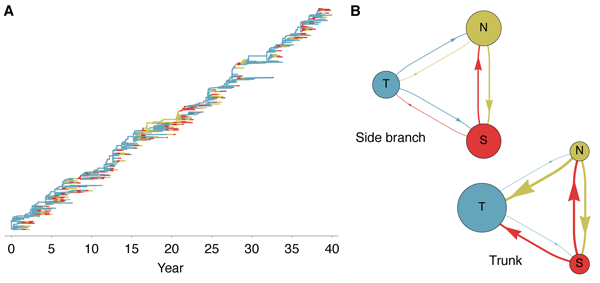
\includegraphics{figures/spatial}
	\caption{\textbf{Patterns of spatial movement of virus lineages}. (A) Evolutionary relationships among 367 viruses sampled evenly through time colored by spatial location. Lineages resides in the north, south and tropics are colored yellow, red and blue respectively. (B) Migration rates between regions on side branch lineages, and (C) Migration rates between regions on trunk lineages. Arrows denote movement of lineages and arrow width is proportional to migration rate. Circle area is proportional to the expected stationary frequency of a region given the observed migration rates.  In both cases, migration rates are calculated across 80 replicate simulations.}
	\label{spatial}
\end{figure}

%%% Figure 5: immunity %%%
\begin{figure}[H]
	\centering
	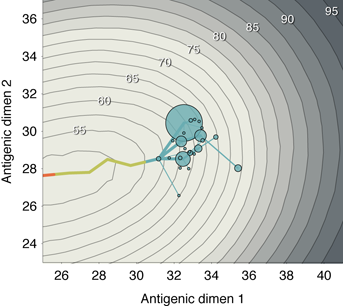
\includegraphics{figures/immunity}
	\caption{\textbf{Host immunity and antigenic history of the virus population}.  Contour lines represent the state of host immunity at the end of the 40-year simulation.  They show the mean risk of infection (as a percentage) after a random host in the population encounters a virus bearing a particular antigenic phenotype.  Contour lines are spaced in intervals of 2.5\%. Bubbles represent a sample of antigenic phenotypes present at the end of the 40-year simulation.  The area of each bubble is proportional to the number of samples with this phenotype.  Lines leading into these bubbles show past antigenic history.  The current phenotypes rapidly coalesce to a trunk phenotype.  The movement of the virus population from top left to the center of the figure can be seen from the antigenic history of the trunk of the virus genealogy. Shifts between antigenic clusters can also be seen as color transitions along the trunk lineage.}
	\label{immunity}
\end{figure}

%%% Figure 6: replicateevol %%%
\begin{figure}[H]
	\centering
	\makebox[\textwidth]{	
		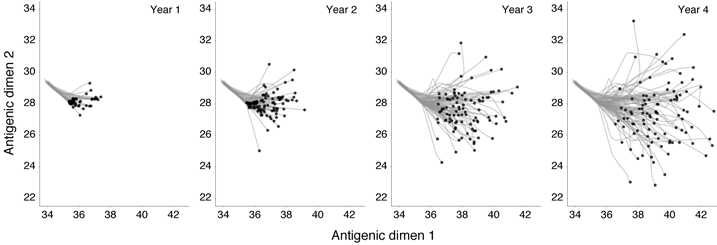
\includegraphics{figures/replicateevol}
	}
	\caption{\textbf{Antigenic phenotypes over the course of 5 years of evolution across 100 replicate simulations starting from identical initial conditions}.  Replicate simulations were initialized with the end state of the original 40-year simulation shown in figures \ref{incmaptree}--\ref{immunity}.  The top left panel shows every antigenic phenotype present in the initial virus population.  The black point represents the population mean.  Each subsequent panel shows an additional year of evolution, with black points representing the mean antigenic phenotypes of the 100 replicate simulations and gray lines representing the history of each mean antigenic phenotype.}
	\label{replicateevol}
\end{figure}


